\documentclass[tikz, border=15pt]{standalone}
\usetikzlibrary{circuits.logic.US, positioning, calc}

\begin{document}
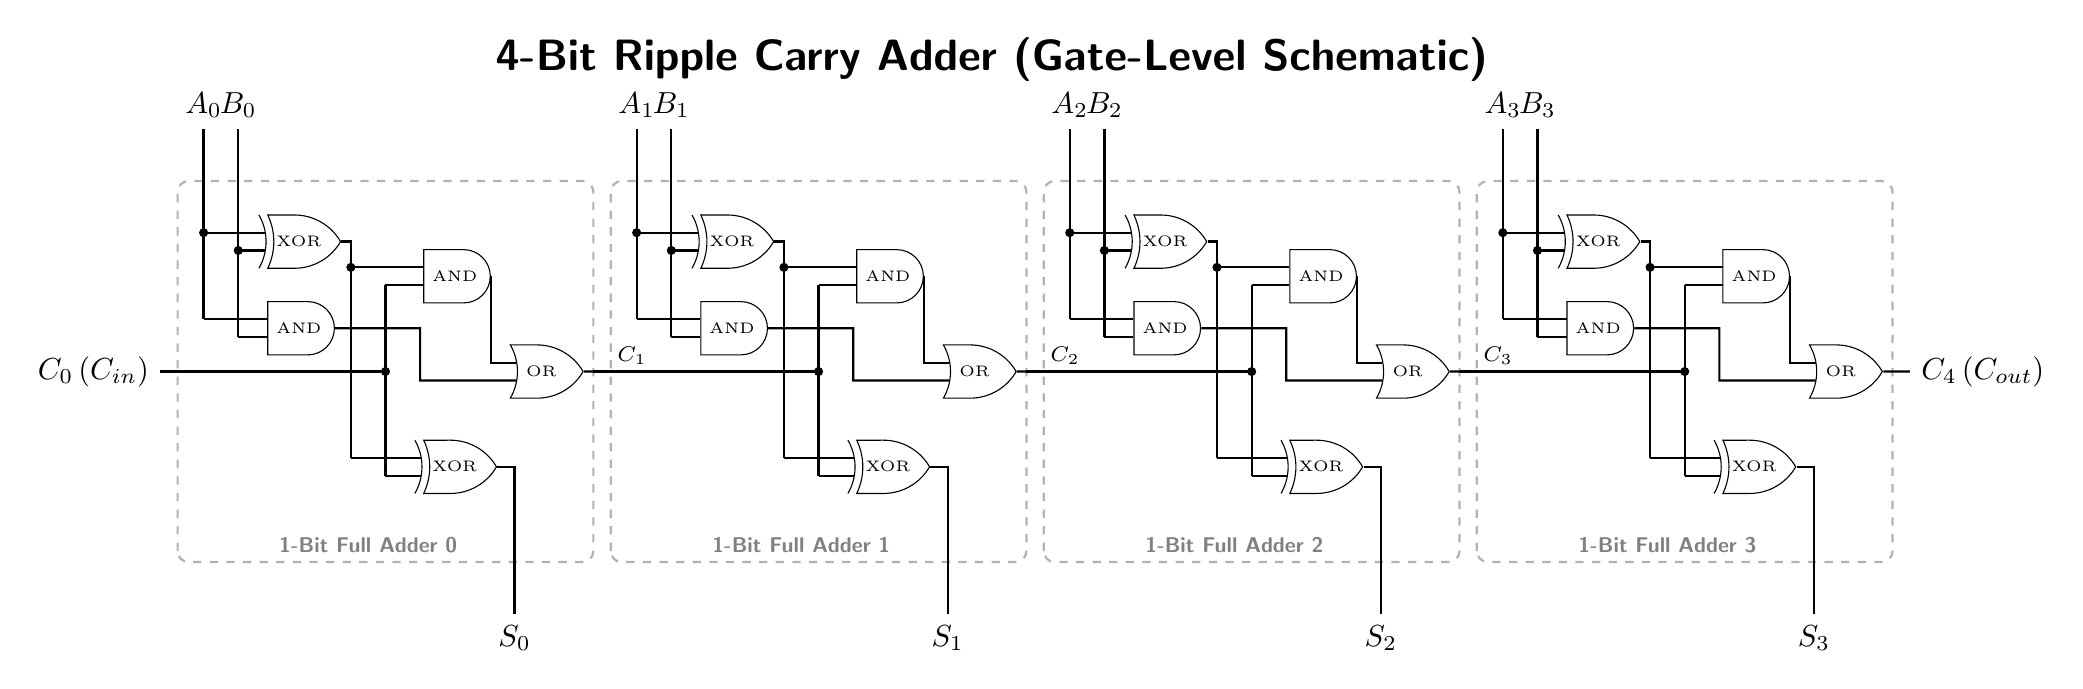
\begin{tikzpicture}[circuit logic US, scale=1.1, every node/.style={transform shape}]

    % 标题
    \node[font=\sffamily\bfseries\Large] at (9.6, 6.0) {4-Bit Ripple Carry Adder (Gate-Level Schematic)};

    % 循环生成 4 个 1位全加器 (从低位 i=0 到高位 i=3)
    \foreach \i [evaluate=\i as \nexti using int(\i+1)] in {0,1,2,3}
    {
        % 计算当前全加器模块的横坐标基准偏移量
        \pgfmathsetmacro{\xframe}{5 * \i}
        
        % 1. 绘制单级全加器的虚线外框
        \draw[dashed, gray!60, thick, rounded corners=4pt] (\xframe + 0.2, 0.2) rectangle (\xframe + 5, 4.6);
        \node[gray, font=\sffamily\bfseries\scriptsize] at (\xframe + 2.4, 0.4) {1-Bit Full Adder \i};

        % 2. 放置该模块内部的 5 个逻辑门
        \node[xor gate, label=center:\tiny XOR] (XOR1_\i) at (\xframe + 1.6, 3.9) {};
        \node[and gate, label=center:\tiny AND] (AND1_\i) at (\xframe + 1.6, 2.9) {};
        \node[and gate, label=center:\tiny AND] (AND2_\i) at (\xframe + 3.4, 3.5) {};
        \node[xor gate, label=center:\tiny XOR] (XOR2_\i) at (\xframe + 3.4, 1.3) {};
        \node[or gate,  label=center:\tiny OR]  (OR1_\i)  at (\xframe + 4.4, 2.4) {};

        % 3. 绘制输入引脚 A_i 和 B_i 及其分支连线
        % A_i 输入及分支
        \draw[thick] (\xframe + 0.5, 5.2) node[above, font=\sffamily] {$A_\i$} -- (\xframe + 0.5, 0 |- AND1_\i.input 1);
        \draw[thick] (\xframe + 0.5, 0 |- XOR1_\i.input 1) -- (XOR1_\i.input 1);
        \fill (\xframe + 0.5, 0 |- XOR1_\i.input 1) circle (1.5pt); 
        \draw[thick] (\xframe + 0.5, 0 |- AND1_\i.input 1) -- (AND1_\i.input 1);

        % B_i 输入及分支
        \draw[thick] (\xframe + 0.9, 5.2) node[above, font=\sffamily] {$B_\i$} -- (\xframe + 0.9, 0 |- AND1_\i.input 2);
        \draw[thick] (\xframe + 0.9, 0 |- XOR1_\i.input 2) -- (XOR1_\i.input 2);
        \fill (\xframe + 0.9, 0 |- XOR1_\i.input 2) circle (1.5pt); 
        \draw[thick] (\xframe + 0.9, 0 |- AND1_\i.input 2) -- (AND1_\i.input 2);

        % 4. 绘制第一个 XOR 门的输出分支 (中间和项)
        \draw[thick] (XOR1_\i.output) -- (\xframe + 2.2, 0 |- XOR1_\i.output) -- (\xframe + 2.2, 0 |- XOR2_\i.input 1);
        \draw[thick] (\xframe + 2.2, 0 |- AND2_\i.input 1) -- (AND2_\i.input 1);
        \fill (\xframe + 2.2, 0 |- AND2_\i.input 1) circle (1.5pt); 
        \draw[thick] (\xframe + 2.2, 0 |- XOR2_\i.input 1) -- (XOR2_\i.input 1);

        % 5. 处理进位链输入 (C_i) 并在模块内部进行分支
        \draw[thick] (\xframe + 2.6, 0 |- AND2_\i.input 2) -- (\xframe + 2.6, 0 |- XOR2_\i.input 2);
        \draw[thick] (\xframe + 2.6, 0 |- AND2_\i.input 2) -- (AND2_\i.input 2);
        \draw[thick] (\xframe + 2.6, 0 |- XOR2_\i.input 2) -- (XOR2_\i.input 2);
        
        % 如果是第 0 级，连接外部输入 C_in
        \ifnum\i=0
            \draw[thick] (\xframe, 2.4) node[left, font=\sffamily] {$C_0\,(C_{in})$} -- (\xframe + 2.6, 2.4);
        \else
            \draw[thick] (\xframe, 2.4) -- (\xframe + 2.6, 2.4);
        \fi
        \fill (\xframe + 2.6, 2.4) circle (1.5pt); 

        % AND2 从输出直下再右折进入 OR.input 1
        \draw[thick] (AND2_\i.output) |- (OR1_\i.input 1);
        % AND1 向右延伸到空旷处(X=3.0)，再下折并水平进入 OR.input 2，完美避开进位总线
        \draw[thick] (AND1_\i.output) -- (\xframe + 3.0, 2.9) |- (OR1_\i.input 2);

        % 使用相对位移 ++(0, -1.7) 确保从 XOR 尖端垂直向下引出
        \draw[thick] (XOR2_\i.output) -- ++(0.2, 0) -- ++(0, -1.7) node[below, font=\sffamily] {$S_\i$};
        
        % 级联进位线连接
        \ifnum\i=3
            % 最后一级输出外部总进位 C_out
            \draw[thick] (OR1_\i.output) -- (\xframe + 5.2, 2.4) node[right, font=\sffamily] {$C_4\,(C_{out})$};
        \else
            % 中间级直接向右延伸
            \draw[thick] (OR1_\i.output) -- (\xframe + 5.7, 2.4) node[above left, font=\sffamily\scriptsize, inner sep=2pt] {$C_{\nexti}$};
        \fi
    }

\end{tikzpicture}
\end{document}